\documentclass[11pt, a4paper]{article}

\usepackage[margin=1in]{geometry}
\usepackage{graphicx}
\usepackage{amsmath, amssymb}
\usepackage{listings}
\usepackage{xcolor}
\usepackage{hyperref}
\usepackage{booktabs}
\usepackage{subcaption}
\usepackage{float}
\usepackage{fancyhdr}
\usepackage{enumitem}

\pagestyle{fancy}
\fancyhf{}
\fancyfoot[C]{\thepage}

\begin{document}

\fancypagestyle{no_hdr_border_rule}{
  \renewcommand{\headrulewidth}{0pt}
}
\thispagestyle{no_hdr_border_rule}

\begin{center}
    {\Large \textbf{Lab 2 -- Report}} \\[0.2cm]
    {\large \textbf{Digital Systems and Microcontrollers (DSM)}} \\[0.1cm]
    {\normalsize International Institute of Information Technology, Hyderabad} \\[0.3cm]
\end{center}

\vspace{0.2cm}
\hrule
\vspace{0.4cm}

\noindent \textbf{Student Name 1:} Manbir Singh Judge \hfill \textbf{Roll Number:} 2026113005 \\
\noindent \textbf{Student Name 2:} Charishma Kandregula \hfill \textbf{Roll Number:} 2026112022 \\
\noindent \textbf{Table Number:} 16 \hfill \textbf{Lab Room Number:} 114 \\
\noindent \textbf{Date of Experiment:} 18/09/2026

\vspace{0.4cm}
\hrule
\vspace{0.5cm}

\vspace{1em}

\tableofcontents
\vspace{0.5cm}
\hrule
\vspace{0.8cm}

\newpage
\fancyhead[L]{Lab 2 -- Report}

% ==============================================================================
% experiment 1
% ==============================================================================

\fancyhead[R]{Experiment 1}
\section{Experiment 1}

\subsection{Aim}

To find out the logic function of each of the given ICs.

\subsection{Components \& Equipment Required}

\begin{itemize}
    \item Digital Test Kit (DTK) -- including power supply, switches, indicator LED pairs and breadboard
    \item \textbf{ICs:} 7486, 7408, 7404, CD4001, CD4011, 7432
    \item Connecting Wires
\end{itemize}

\subsection{Procedure}

\begin{itemize}
    \item Mount the ICs 7486, 7408, 7404 across the center notch of the breadboard.
    \item For each IC, connect Pin 14 ($V_{CC}$) to the power rail and Pin 7 ($\text{GND}$) to the ground rail.
    \item For each IC, connect input pins of one of the gates to switches on the DTK.
    \item For each IC, connect the output pin of the above gate to one of the indicator LED pairs.
    \item Observe and note the output of each IC for all four combinations of inputs.
    \item Repeat the above steps for ICs CD4001, CD4011, 7432.
\end{itemize}

\subsection{Observations}

\begin{minipage}[t]{0.48\textwidth}

\begin{table}[H]
    \centering
    \caption{Observation for IC 7486}
    \begin{tabular}{|c|c|c|}
        \hline
        $A_1$ & $B_1$ & Output \\
        \hline
        0 & 0 & 0 \\
        \hline
        0 & 1 & 1 \\
        \hline
        1 & 0 & 1 \\
        \hline
        1 & 1 & 0 \\
        \hline
    \end{tabular}
\end{table}

\begin{table}[H]
    \centering
    \caption{Observation for IC 7408}
    \begin{tabular}{|c|c|c|}
        \hline
        $A_1$ & $B_1$ & Output \\
        \hline
        0 & 0 & 0 \\
        \hline
        0 & 1 & 0 \\
        \hline
        1 & 0 & 0 \\
        \hline
        1 & 1 & 1 \\
        \hline
    \end{tabular}
\end{table}

\begin{table}[H]
    \centering
    \caption{Observation for IC 7404}
    \begin{tabular}{|c|c|}
        \hline
        Input & Output \\
        \hline
        0 & 1 \\
        \hline
        1 & 0 \\
        \hline
    \end{tabular}
\end{table}

\end{minipage}
\hfill
\begin{minipage}[t]{0.48\textwidth}
    
\begin{table}[H]
    \centering
    \caption{Observation for IC CD4001}
    \begin{tabular}{|c|c|c|}
        \hline
        $A_1$ & $B_1$ & Output \\
        \hline
        0 & 0 & 1 \\
        \hline
        0 & 1 & 0 \\
        \hline
        1 & 0 & 0 \\
        \hline
        1 & 1 & 0 \\
        \hline
    \end{tabular}
\end{table}

\begin{table}[H]
    \centering
    \caption{Observation for IC CD4011}
    \begin{tabular}{|c|c|c|}
        \hline
        $A_1$ & $B_1$ & Output \\
        \hline
        0 & 0 & 1 \\
        \hline
        0 & 1 & 1 \\
        \hline
        1 & 0 & 1 \\
        \hline
        1 & 1 & 0 \\
        \hline
    \end{tabular}
\end{table}

\begin{table}[H]
    \centering
    \caption{Observation for IC 7432}
    \begin{tabular}{|c|c|c|}
        \hline
        $A_1$ & $B_1$ & Output \\
        \hline
        0 & 0 & 0 \\
        \hline
        0 & 1 & 1 \\
        \hline
        1 & 0 & 1 \\
        \hline
        1 & 1 & 1 \\
        \hline
    \end{tabular}
\end{table}

\end{minipage}

\subsection{Tinkercad Simulation}
\noindent \textbf{Tinkercad Link:} \href{https://www.tinkercad.com/things/kATGKwCnRwN-dms-lab-2-exp-1?sharecode=7HgT0J6fQ6QNoWgAy2pFz0Ol8pav9oxKmdrKJmCbqXE}{\color{blue}Click here}
\begin{figure}[H]
\centering
    \centering
    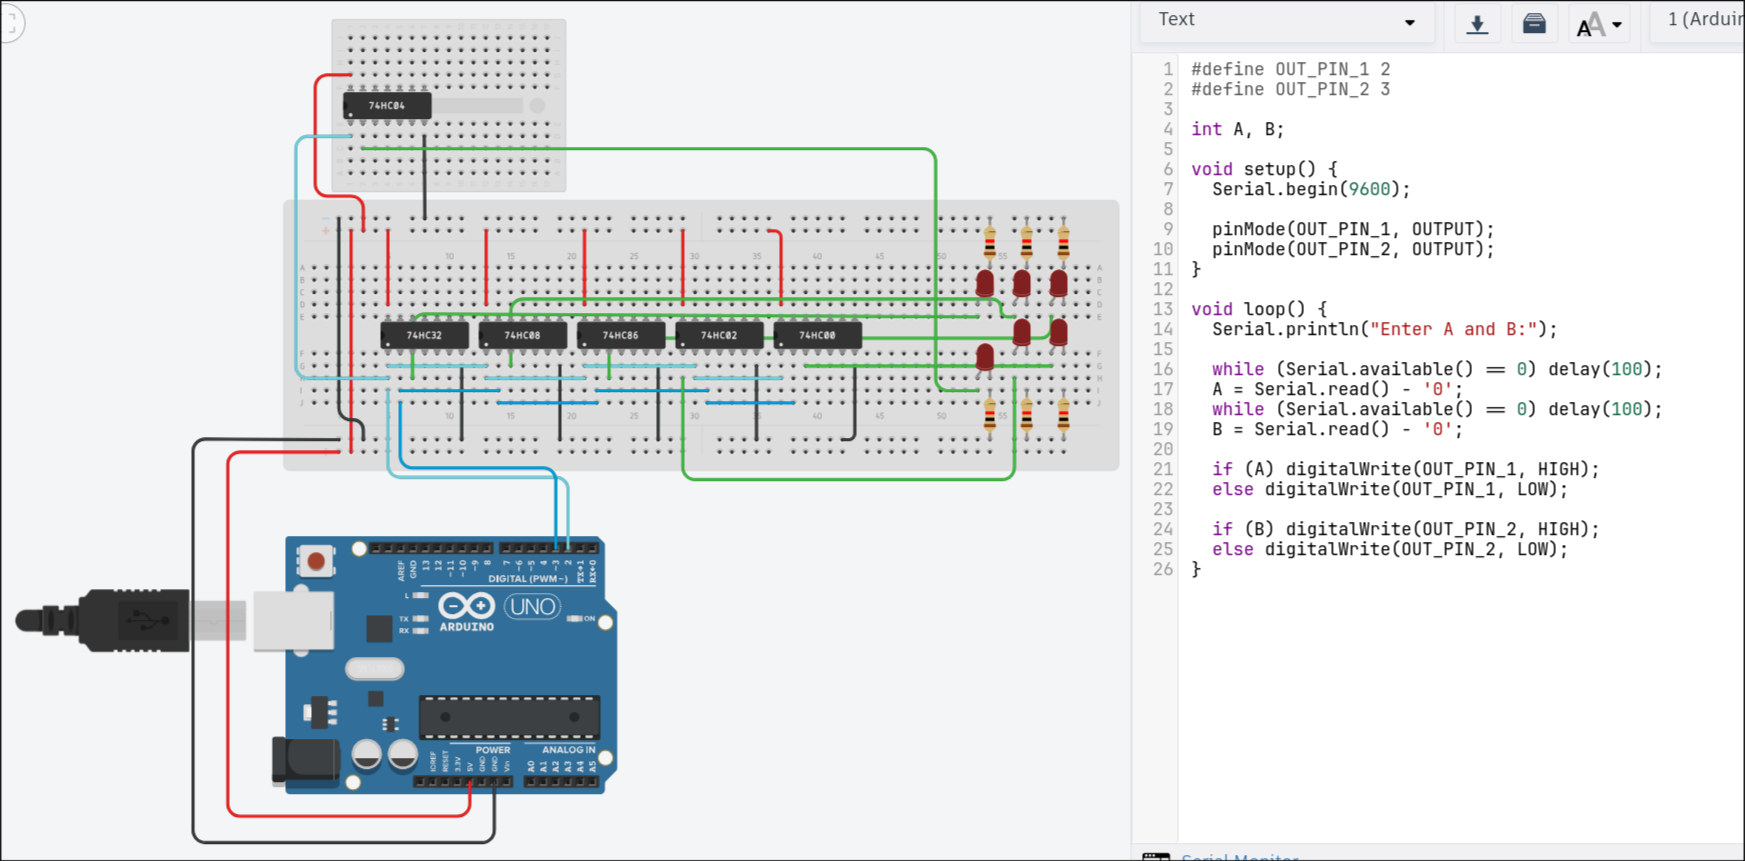
\includegraphics[width=\textwidth]{tc1.png}
    \caption{Tinkercad Simulation Screenshot}
\end{figure}

\subsection{Hardware Setup Photograph}
\begin{figure}[H]
    \centering
    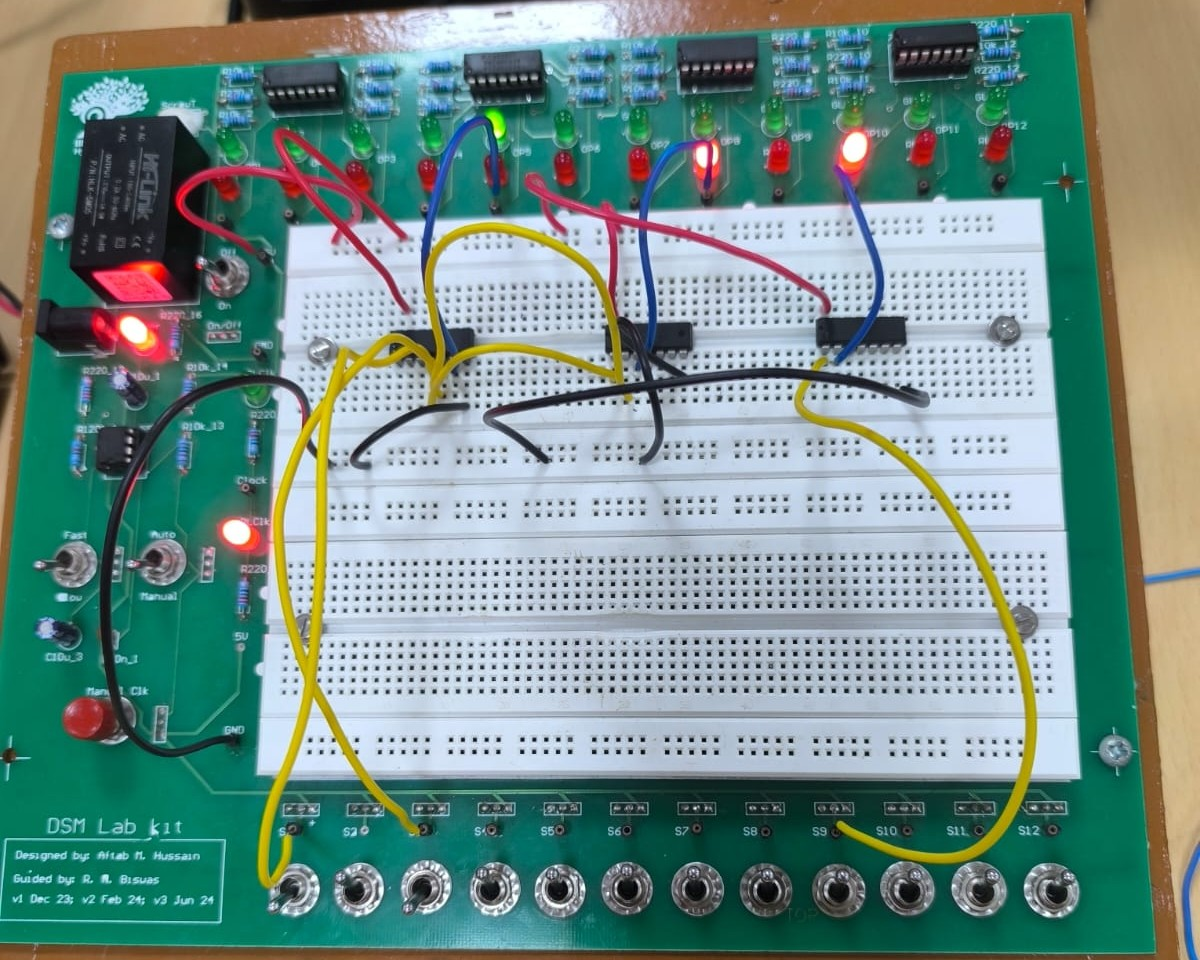
\includegraphics[width=0.6\textwidth]{lab1.jpeg}
    \caption{IC 7486, IC 7408, IC 7404 (left-to-right)}
\end{figure}
\begin{figure}[H]
    \centering
    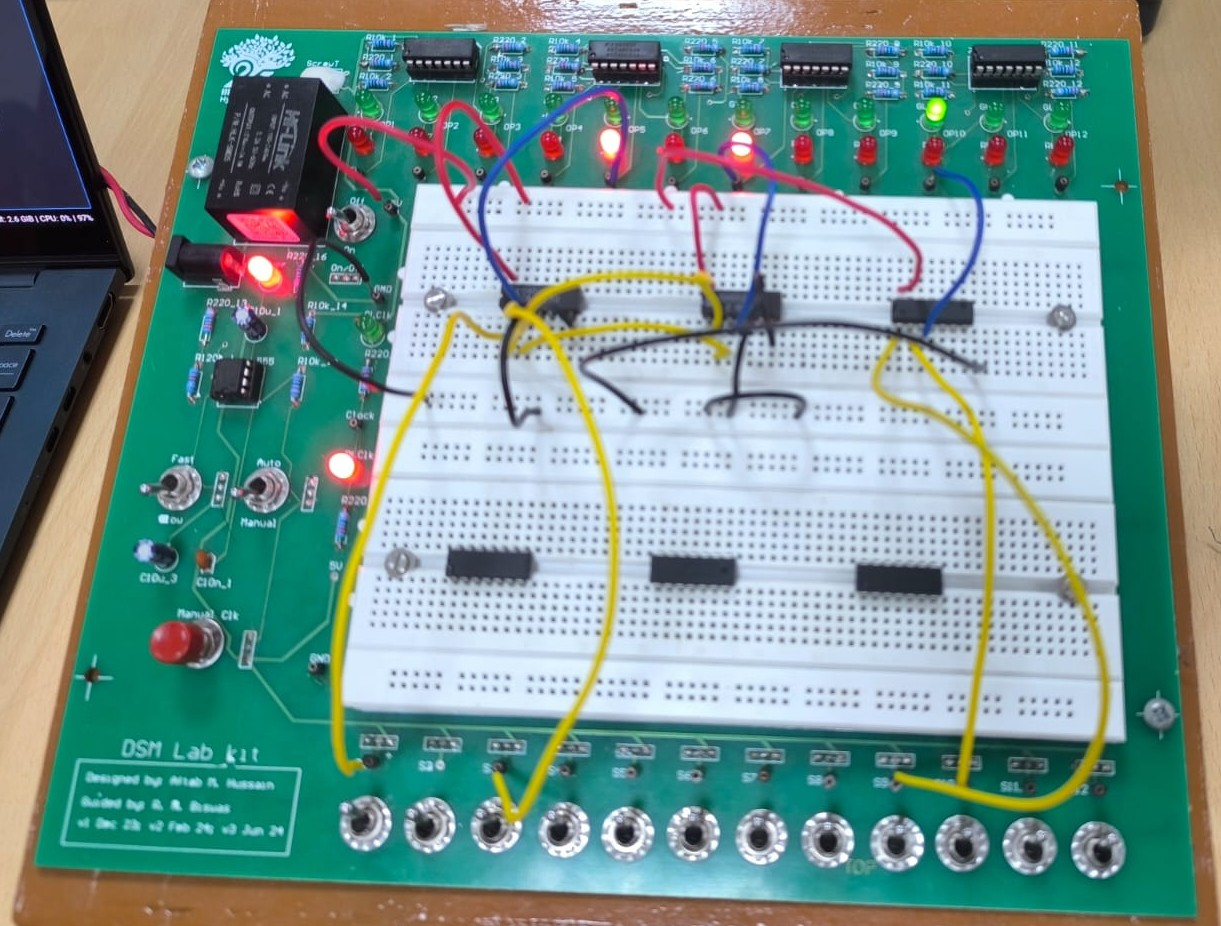
\includegraphics[width=0.6\textwidth]{lab2.jpeg}
    \caption{IC CD4001, IC CD4011, IC 7432 (left-to-right)}
\end{figure}

\subsection{Conclusion}
\begin{itemize}
    \item Logic function of IC 7486 is identified XOR (as expected).
    \item Logic function of IC 7408 is identified AND (as expected).
    \item Logic function of IC 7404 is identified NOT (as expected).
    \item Logic function of IC CD4001 is identified NOR (as expected).
    \item Logic function of IC CD4011 is identified NAND (as expected).
    \item Logic function of IC 7432 is identified OR (as expected).
    \item \textbf{Summary:} Logic function of all ICs were as expected.
\end{itemize}

\newpage

% ==============================================================================
% experiment 2
% ==============================================================================

\fancyhead[R]{Experiment 2}
\section{Experiment 2}

\subsection{Aim}
Verification of De Morgan's Laws:
\begin{itemize}
    \item $\overline{A \cdot B} = \overline{A} + \overline{B}$
    \item $\overline{A + B} = \overline{A} \cdot \overline{B}$
\end{itemize}

\subsection{Components \& Equipment Required}
\begin{itemize}
    \item Digital Test Kit (DTK) -- including power supply, switches, indicator LED pairs and breadboard
    \item \textbf{ICs:} 7408-AND, CD4001-NOR, CD4011-NAND, 7432-OR
    \item Connecting Wires
\end{itemize}

\subsection{Procedure}
\begin{enumerate}[label=\textbf{(\alph*)}]
    \item \textbf{Verification of $\overline{A \cdot B} = \overline{A} + \overline{B}$:}
    \begin{itemize}
        \item Set up the ICs CD4011-NAND and 7432-OR.
        \item Generate the complements of inputs $A$ and $B$ using 2 NAND gates in IC CD4011 using the relation $\overline{A \cdot A}=\overline{A}$.
        \item Connect the complemented inputs from above NAND gates to one of the OR gate in IC 7432. The output of this OR gate is RHS; connect it to an indicator LED pair on DKT.
        \item Connect the inputs $A$ and $B$ into one of the NAND gates in IC CD4011. Output of this NAND gate is our LHS (i.e., the direct output); connect it to an indicator LED pair on DKT.
        \item Observe and note the outputs.
    \end{itemize}
    \item \textbf{Verification of $\overline{A + B} = \overline{A} \cdot \overline{B}$:}
    \begin{itemize}
        \item Set up the ICs 7408-AND, CD4001-NOR and CD4011-NAND.
        \item Generate the complements of inputs $A$ and $B$ using 2 NAND gates in IC CD4011 using the relation $\overline{A \cdot A}=\overline{A}$.
        \item Connect the complemented inputs from above NAND gates to one of the AND gate in IC 7408. The output of this AND gate is RHS; connect it to an indicator LED pair on DKT.
        \item Connect the inputs $A$ and $B$ into one of the NOR gates in IC CD4001. Output of this NOR gate is our LHS (i.e., the direct output); connect it to an indicator LED pair on DKT.
        \item Observe and note the outputs.
    \end{itemize}
\end{enumerate}


\subsection{Observations}
\begin{table}[H]
    \centering
    \caption{Observation for $\overline{A \cdot B} = \overline{A} + \overline{B}$}
    \begin{tabular}{|c|c|c|c|}
        \hline
        $A$ & $B$ & $\overline{A \cdot B}$ (LHS) & $\overline{A} + \overline{B}$ (RHS) \\
        \hline
        0 & 0 & 1 & 1 \\
        \hline
        0 & 1 & 1 & 1 \\
        \hline
        1 & 0 & 1 & 1 \\
        \hline
        1 & 1 & 0 & 0 \\
        \hline
    \end{tabular}
\end{table}
\begin{table}[H]
    \centering
    \caption{Observation for $\overline{A + B} = \overline{A} \cdot \overline{B}$}
    \begin{tabular}{|c|c|c|c|}
        \hline
        $A$ & $B$ & $\overline{A + B}$ (LHS) & $\overline{A} \cdot \overline{B}$ (RHS) \\
        \hline
        0 & 0 & 1 & 1 \\
        \hline
        0 & 1 & 0 & 0 \\
        \hline
        1 & 0 & 0 & 0 \\
        \hline
        1 & 1 & 0 & 0 \\
        \hline
    \end{tabular}
\end{table}

\subsection{Tinkercad Simulation}
\noindent \textbf{Tinkercad Link:} \href{https://www.tinkercad.com/things/lKgbpBDrOE0-dms-lab-2-exp-2?sharecode=7S5MEHwnXGBaEBTygyPoW4ldG7CQEkxFdRFCpr8eibA}{\color{blue}Click here}
\begin{figure}[H]
\centering
    \centering
    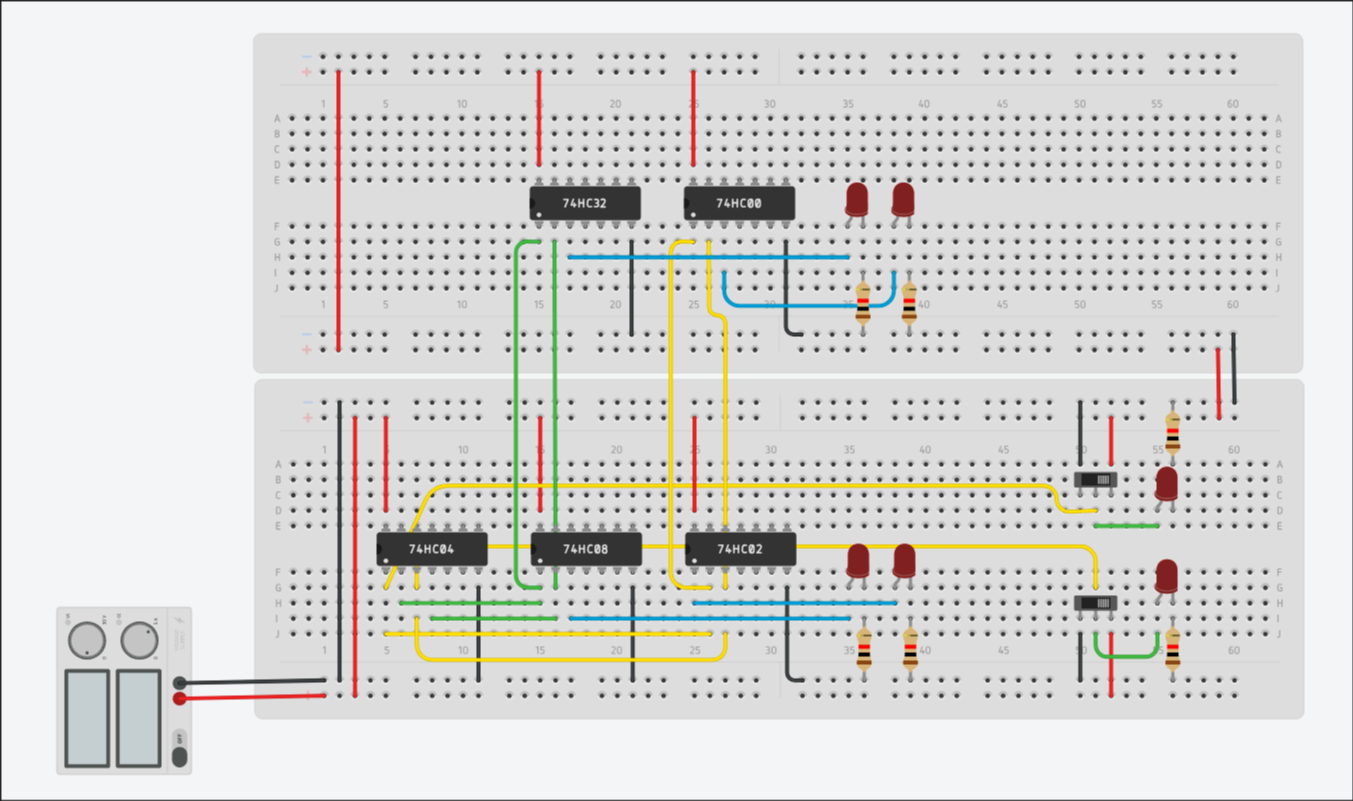
\includegraphics[width=\textwidth]{tc2.png}
    \caption{Tinkercad Simulation Screenshot}
\end{figure}

\subsection{Hardware Setup Photograph}
\begin{figure}[H]
    \centering
    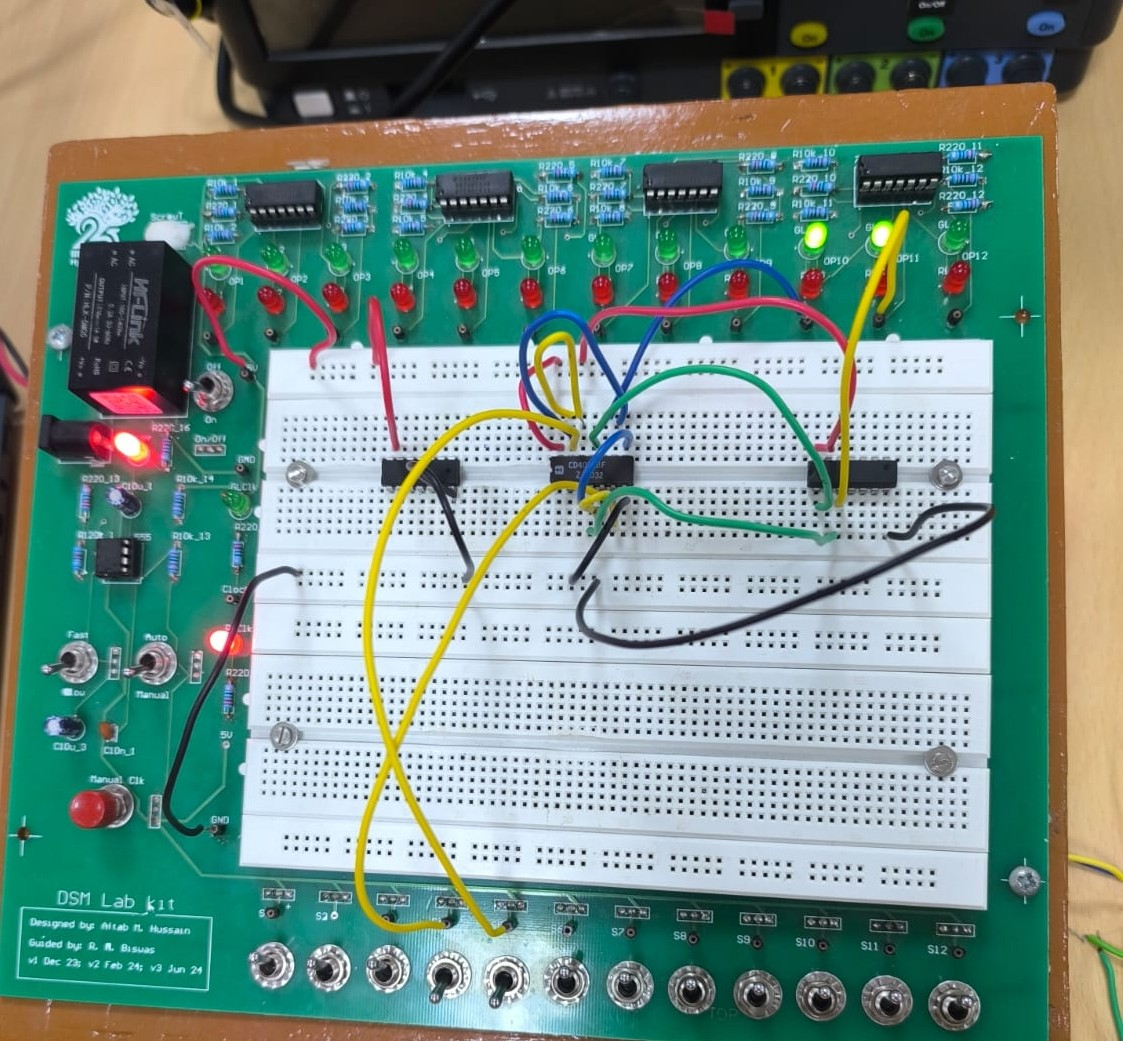
\includegraphics[width=0.6\textwidth]{lab3.jpeg}
    \caption{Hardware Setup for part (a) \\ ICs: 7408 (unused), CD4011-NAND, 7432-OR}
\end{figure}
\begin{figure}[H]
    \centering
    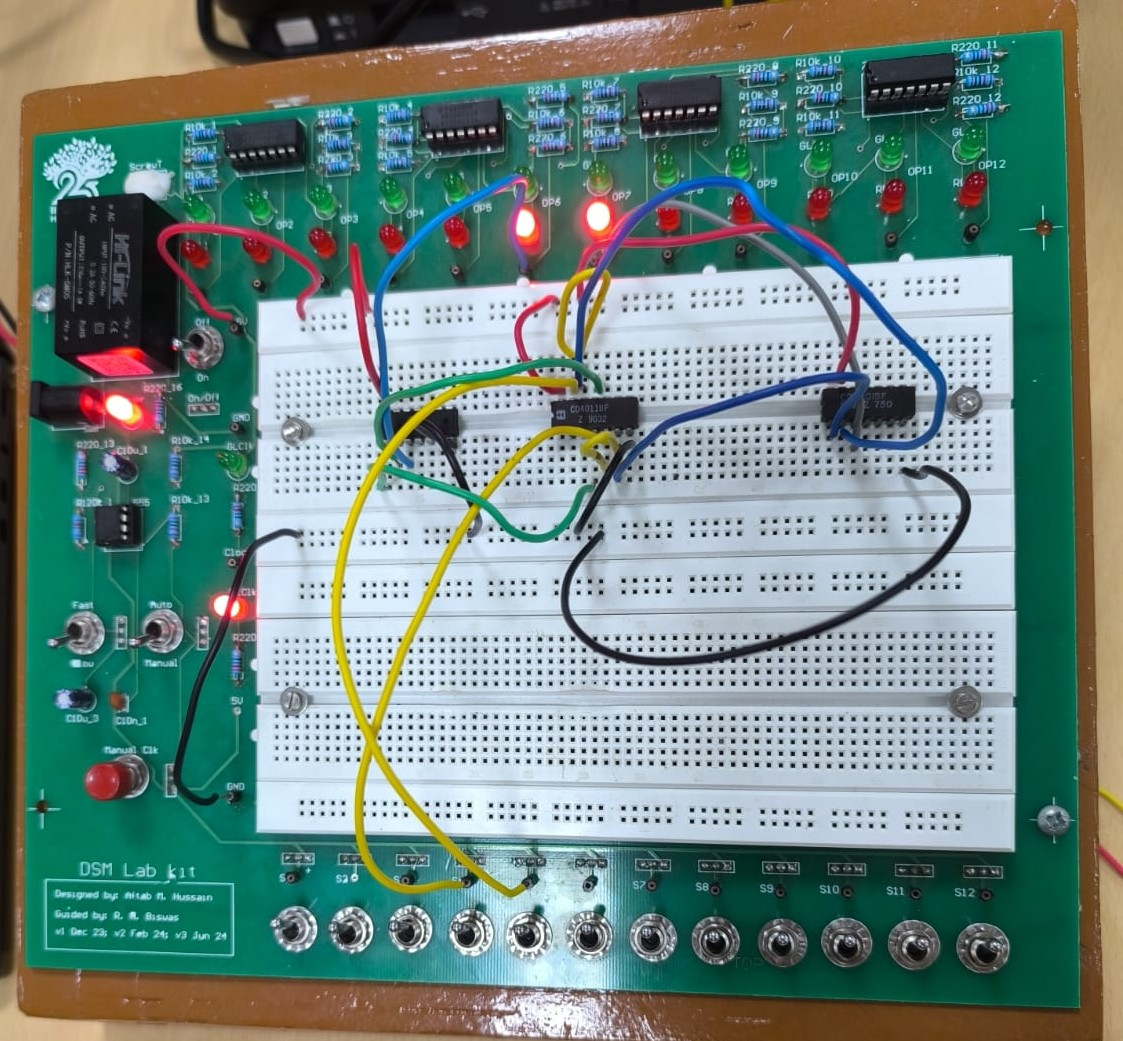
\includegraphics[width=0.6\textwidth]{lab4.jpeg}
    \caption{Hardware Setup for part (b) \\ ICs: 7408-AND, CD4011-NAND, CD4001-NOR}
\end{figure}

\subsection{Conclusion}
De Morgan's laws are verified.

\end{document}